\title{\myfont Narrative of Analysis for Time Series Consideration in Diabetes Predictors
}

\date{\today}

\documentclass{article}

\usepackage{setspace}
\usepackage{etoolbox}
\usepackage{caption}
\setlength\parindent{24pt}
\usepackage{subfig}
\usepackage{fullpage}
\usepackage{graphicx}
\usepackage{amsmath}
\usepackage{amssymb}
\usepackage{color}
\usepackage{gensymb}
\usepackage{tabularx}
\usepackage{tikz}
\usetikzlibrary{fit,positioning,arrows,automata,calc}
\tikzset{
  main/.style={circle, minimum size = 5mm, thick, draw =black!80, node distance = 10mm},
  connect/.style={-latex, thick},
  box/.style={rectangle, draw=black!100}
}
\usepackage{tikz-qtree}
\usepackage{floatrow}
\usepackage{subfig}
\usepackage{hyperref}
\hypersetup{
    colorlinks=true,
    linkcolor=blue,
    filecolor=magenta,      
    urlcolor=brown,
}


\begin{document}
\font\myfont=cmr12 at 16pt
\maketitle


\section{Why Is this Useful? How can we improve on previous Approaches?}

- Comorbidity of diabetes with other things: micro/macro complications. Give medical details.

- What has been done in the past. Find a problem similar to this. What is the best model used so far? Has anyone done this with claims data? It'll probably be logistic regression on a small research cohort. What kind of metrics are they using? AUC and Accuracy? F1 measure?

\section{The Question, The Process}
\doublespacing

We seek to explore the efficacy in considering the timing of tests, diagnoses, and conditions in health insurance claims on predicting whether a patient has diabetes or not. Approaching this subject will involve gradual steps. Working with the data from $\approx$ 43,000,000 people who have health insurance claims through Aetna, we seek to extract predictors of diabetes from the variety of ICD and CPT filings in these records. 
 

\subsection{Time Independent Diabetes Predictors}

Before trying to extract time-related information regarding whether a patient has diabetes, we want to establish that there are inherent predictors in the Aetna database for having diabetes. We want to establish which of these predictors is the most effective in suggesting diabetes. 

\subsubsection{Data for initial steps}

We will create a sparse feature matrix across subjects that will indicate the issuance or non-issuance of certain tests/screenings. We will take a population of patients such that there are some with diabetes and some without, and seek to work with hetergenous data -- not specific to location, race, gender, etc. Each patient will be a row in the feature matrix, and each column will indicate the presence or absence of one of the tests. 


\subsubsection{Model Fitting} 
Since the data are quite categorical, and the final conclusion is as well, perhaps a logistic regression or SVM/margin based classifer would be useful for this classification (for soft margin/hard margin info: \href{https://github.com/harvard-ml-courses/cs181-lectures/blob/master/10.handout.pdf}{here}). \begin{itemize}

\item The relative quality of the logistic regression model can be measured with an Akaike information criterion (AIC) for it, defined as: $ \textrm{AIC} = 2k - 2 \ln L$, where k is the number of features and L is the likelihood function. We seek to maximize the log likelihood of the data (for computation purposes this is easier) where L is: \begin{gather}
\ln L(\mathbf{w} | \mathbf{X}) = \prod_{i} \ln P(y_i |\mathbf{x}_i, \mathbf{w}) = \prod_{i} \ln(\sigma(\mathbf{w},\mathbf{x}_i)^{y_i} (1 - \sigma(\mathbf{w},\mathbf{x}_i))^{1-y_i} ,  \\  \textrm{where}  \quad \sigma(\mathbf{w},\mathbf{x}) = \frac{1}{1 +e^{-\mathbf{w}^T \mathbf{x}}} \qquad
\end{gather}

One can either maximize the this function, or minimize the negative of it, essentially asking how likely are the regression parameters $\mathbf{w}$ given the data $\mathbf{X}$?

\item The SVM approach with a soft margin involves minimizes the loss defined as:
\begin{equation}
\mathcal{L} = \frac{1}{n} [\sum_{i=1}^{n} \max{0, 1-y_i (\mathbf{w} \cdot \mathbf{x} - b) }] + \lambda ||\mathbf{w}||^2
\end{equation}

where b is the coordinate intercept for hyperplanes at $\mathbf{w} \cdot \mathbf{x} - b = 0$ and the $\lambda$ is penalizing term for overfitting weight coefficients.
\end{itemize}
Both of these can be optimized with gradient descent to find the optimum weights to (a) maximize likelihood or (b) minimize loss.

The steps above help to optimize the weights for maximum predictability. We can see which features have the most influence on finding the maximum likelihood or minimum loss by withholding them iteratively and seeing how that influences the optimization. One thing to consider is that the features could be correlated, and removing one will not have as great an impact as removing them both, for example. It would be hard to quantify which are correlated with this method. Will have to think more about this. 

\subsubsection{Tests}

Measure of accuracy depends on what it will be used for?

\begin{itemize}
\item Where do you want to be on ROC curve? 
\item We would rather have false positives. High sensitivity with less specificity. 
\item AUC, accuracy 
\item Doctors love full explanations of metrics. Think about that while we target these journals (JAMA has been emphasizing data science approaches) Look up JAMA 2016 Diabetic Retinopathy
\end{itemize}

\subsection{Initial Test of Time Dependence}

We want to see if some of these ICD and CPT filings can be used ahead of time to predict that diabetes will be onset later. As an initial test, we can see if there is a correlation between future diabetes diagnosis and the presence of some of the highly indicating features we derived from above appearing earlier in their health insurance claims.

\subsubsection{Data}

We want to look at patients with continuous health insurance claims from 2012-2013. We want to mitigate enrollment bias and bias from patients that appear in the claims file right as they are diagnosed with diabetes, for example (nothing to really predict there, but they are useful for the previous step). 

\subsubsection{Tests}

Eventually, we would like to implement a method that infer what state the patient is in (diabetic, non-diabetic) as a latent variable. Using a hidden markov model, information about the observables of a patient at an earlier time can be used to infer what "state" the patient is in at later times or what state they were in at earlier times. We can employ this technique in intervals of years or whatever the smallest continuous increment of health insurance claims are with a viable data set size.
\begin{figure}
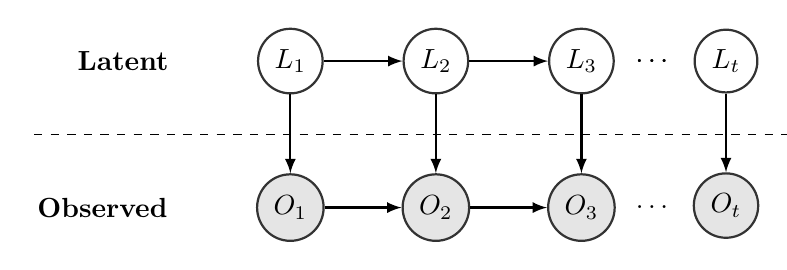
\begin{tikzpicture}
  \node[box,draw=white!100] (Latent) {\textbf{Latent}};
  \node[main] (L1) [right=of Latent] {$L_1$};
  \node[main] (L2) [right=of L1] {$L_2$};
  \node[main] (L3) [right=of L2] {$L_3$};
  \node[main] (Lt) [right=of L3] {$L_t$};
  \node[main,fill=black!10] (O1) [below=of L1] {$O_1$};
  \node[main,fill=black!10] (O2) [below=of L2] {$O_2$};
  \node[main,fill=black!10] (O3) [below=of L3] {$O_3$};
  \node[main,fill=black!10] (Ot) [below=of Lt] {$O_t$};
  \node[box,draw=white!100,left=of O1] (Observed) {\textbf{Observed}};
  \path (L3) -- node[auto=false]{\ldots} (Lt);
  \path (L1) edge [connect] (L2)
        (L2) edge [connect] (L3)
        (L3) -- node[auto=false]{\ldots} (Lt);
  \path (O1) edge [connect] (O2)
        (O2) edge [connect] (O3)
        (O3) -- node[auto=false]{\ldots} (Ot);
  \path (L1) edge [connect] (O1);
  \path (L2) edge [connect] (O2);
  \path (L3) edge [connect] (O3);
  \path (Lt) edge [connect] (Ot);

  % draw the dashed line
  \draw [dashed, shorten >=-1cm, shorten <=-1cm]
      ($(Latent)!0.5!(Observed)$) coordinate (a) -- ($(Lt)!(a)!(Ot)$);
\end{tikzpicture}
\caption{Diagram of HMM. $\mathit{L}_t$ is a sparse state vector corresponding to either not diabetic or diabetic, where the subscript is the time interval (for example, 1 is 2012, 2 is 2013). $\mathit{O}_t$ is the feature vector -- what we observe in the patient at time $t$. }
\end{figure}

The quality of this model can be measured using the forward and backward algorithms (Baum-Welch) on test data to maximize likelihood. If not with that, we can use the Viterbi algorithm.

(Explain VITERBI Algorithm)



This circumstance will require some exploration. An initial sense of how granular the data can be will be important. That is, if we would like to use a model to predict the latent state of a patient as diabetic or not, how closely positioned are the time intervals on which we define states? Will there be enough people who have continuous data on, say, the month resolution, to label states that acutely? Does the absence of information inform us of diabetic state for a patient? These questions will be examined.

\subsubsection{Utility}

It is important to know if such granularity can be achieved to properly answer an overarching question: can these claims be used to develop a predictor of diabetes that precedes the diagnosis in the health insurance claims, and how much earlier can such a prediction be made for individuals?

\section{Objectives in 4 steps}

\begin{enumerate}
\item The first objective is to create a non-temporal classifier of diabetes. We will test this using a logistic regression. If that works well, we will also examine the accuracy of an SVM in doing this as well. This is a test to see what variables are most acutely tied to patients having diabetes. We suspect that this will work well, and we will get a variety of categorical variables (or perhaps some continuous ones from pharmacology) that are indicative of diabetes. We can also look for variables that are most acutely associated with people who are not diabetic.

\item Once we have these variables we would like to explore whether the presence of some of these when patients don't have a diabetes claim in 2012 is correlated to them getting diabetes the following year. This may be a better point for model optimization (figuring out which variables are most robust in predicting that transition).  There are \textbf{four state transitions that we are possible that we care about}: 

\begin{itemize}
\item We want to know when someone who wasn't diabetic becomes diabetic and want to be able to predict that. This is the first priority. We hope to find that the people who make this transition have a pretty related set of indicators that indicate their transition. Granularity of a year, though, may not be able to fully capture this. Hopefully it can if we look at ALL tests/pharma/diag in that year.

\item We also want to know when someone who was diabetic is no longer the following year. This transition as defined as when a year of contiguous Aetna enrollment with $<$ 2 outpatient claims (HEDIS criteria). \textbf{Question for Arjun: which type of outpatient claims are we referring to here?}

\item These indicator variables will hopefully also capture patients who were diabetic in 2012 and remain so in 2013. 

\item The last circumstance is that someone who is not diabetic remains not diabetic. 
\end{itemize}

\item 	The interval of time of just a year may not be as resolved as we like, so what we can do is expand this from 2011 to 2014. This will help us explore the variety of 

\item From here, we want to implement the HMM model to qualify the transition probabilities of the four states mentioned in item 2. This is where we want to understand what features most drastically influence these transition probabilities. 
\end{enumerate}

\end{document}